%iffalse           
\let\negmedspace\undefined
\let\negthickspace\undefined
\documentclass[journal,12pt,onecolumn]{IEEEtran}
\usepackage{cite}
\usepackage{amsmath,amssymb,amsfonts,amsthm}
\usepackage{algorithmic}
\usepackage{graphicx}
\usepackage{textcomp}
\usepackage{xcolor}
\usepackage{txfonts}
\usepackage{listings}
\usepackage{enumitem}
\usepackage{mathtools}
\usepackage{gensymb}
\usepackage{comment}
\usepackage[breaklinks=true]{hyperref}
\usepackage{tkz-euclide} 
\usepackage{listings}
\usepackage{gvv}                                        
\def\inputGnumericTable{}                                 
\usepackage[latin1]{inputenc}                                
\usepackage{color}                                            
\usepackage{array}                                            
\usepackage{longtable}                                       
\usepackage{calc}                                             
\usepackage{multirow}                                         
\usepackage{hhline}                                           
\usepackage{ifthen}                                           
\usepackage{lscape}

\newtheorem{theorem}{Theorem}[section]
\newtheorem{problem}{Problem}
\newtheorem{proposition}{Proposition}[section]
\newtheorem{lemma}{Lemma}[section]
\newtheorem{corollary}[theorem]{Corollary}
\newtheorem{example}{Example}[section]
\newtheorem{definition}[problem]{Definition}
\newcommand{\BEQA}{\begin{eqnarray}}
\newcommand{\EEQA}{\end{eqnarray}}
\newcommand{\define}{\stackrel{\triangle}{=}}
\theoremstyle{remark}
\newtheorem{rem}{Remark}
\usepackage{circuitikz}
\begin{document}

\bibliographystyle{IEEEtran}
\vspace{3cm}
\title{9-9.2-40}
\author{EE24BTECH11052 - RONGALI CHARAN}
% \maketitle
% \newpage
% \bigskip
{\let\newpage\relax\maketitle}

\renewcommand{\thefigure}{\theenumi}
\renewcommand{\thetable}{\theenumi}
\setlength{\intextsep}{10pt} % Space between text and floats


\numberwithin{equation}{enumi}
\numberwithin{figure}{enumi}
\renewcommand{\thetable}{\theenumi}
\textbf{Question:} The area of the region bounded by the curve $y=\sqrt{16-x^2}$ and $x$-axis is
\begin{enumerate}
\item $8\pi$ sq units
\item $20\pi$ sq units
\item $16\pi$ sq units
\item $256\pi$ sq units
\end{enumerate}
\solution
The equation of conic $g(x)$ is given by :
\begin{align}
	g(x) &= \vec{x}^\top \vec{V}\vec{x}+2\vec{u}^\top \vec{x}+f=0\\
	\vec{V} &= \myvec{1 & 0\\0 & 1}\\
	\vec{u} &= \myvec{0 \\ 0} \\
	f &= -16\\
	L: \vec{x} &= \vec{h}+k\vec{m} \\
	\vec{h} &= \myvec{x \\ 0}\\
	\vec{m} &= \myvec{1 \\ 0}\\
	\vec{x_i} &= \vec{h}+k_{i}\vec{m}
       \end{align}
\begin{align}
	k_1 &= \frac{1}{\vec{m}^\top \vec{V}\vec{m}}\brak{-m^\top\brak{\vec{V}\vec{h}+\vec{u}}+ \sqrt{[\vec{m}^\top \brak{\vec{V}\vec{h}+\vec{u}}]^2 - g(\vec{h})\brak{\vec{m}^\top\vec{V}\vec{m}}}} = -x+4 \\
	k_2 &= \frac{1}{\vec{m}^\top \vec{V}\vec{m}}\brak{-m^\top\brak{\vec{V}\vec{h}+\vec{u}}- \sqrt{[\vec{m}^\top \brak{\vec{V}\vec{h}+\vec{u}}]^2 - g(\vec{h})\brak{\vec{m}^\top\vec{V}\vec{m}}}} = -x-4
\end{align}
\begin{align}
	\vec{x_1} &= \myvec{4 \\0}\\
	\vec{x_2} &= \myvec{-4\\0}
\end{align}
The area bounded by the curve $y = 16-x^2$ and $x$-axis is given by:
\begin{align}
	\int_{-4}^{4}\brak{\sqrt{16-x^2} }dx &= 8\pi 
\end{align}
Hence, the area bounded by the curve and the line is $8\pi$ sq units.\\
\begin{figure}[h]
	\centering
	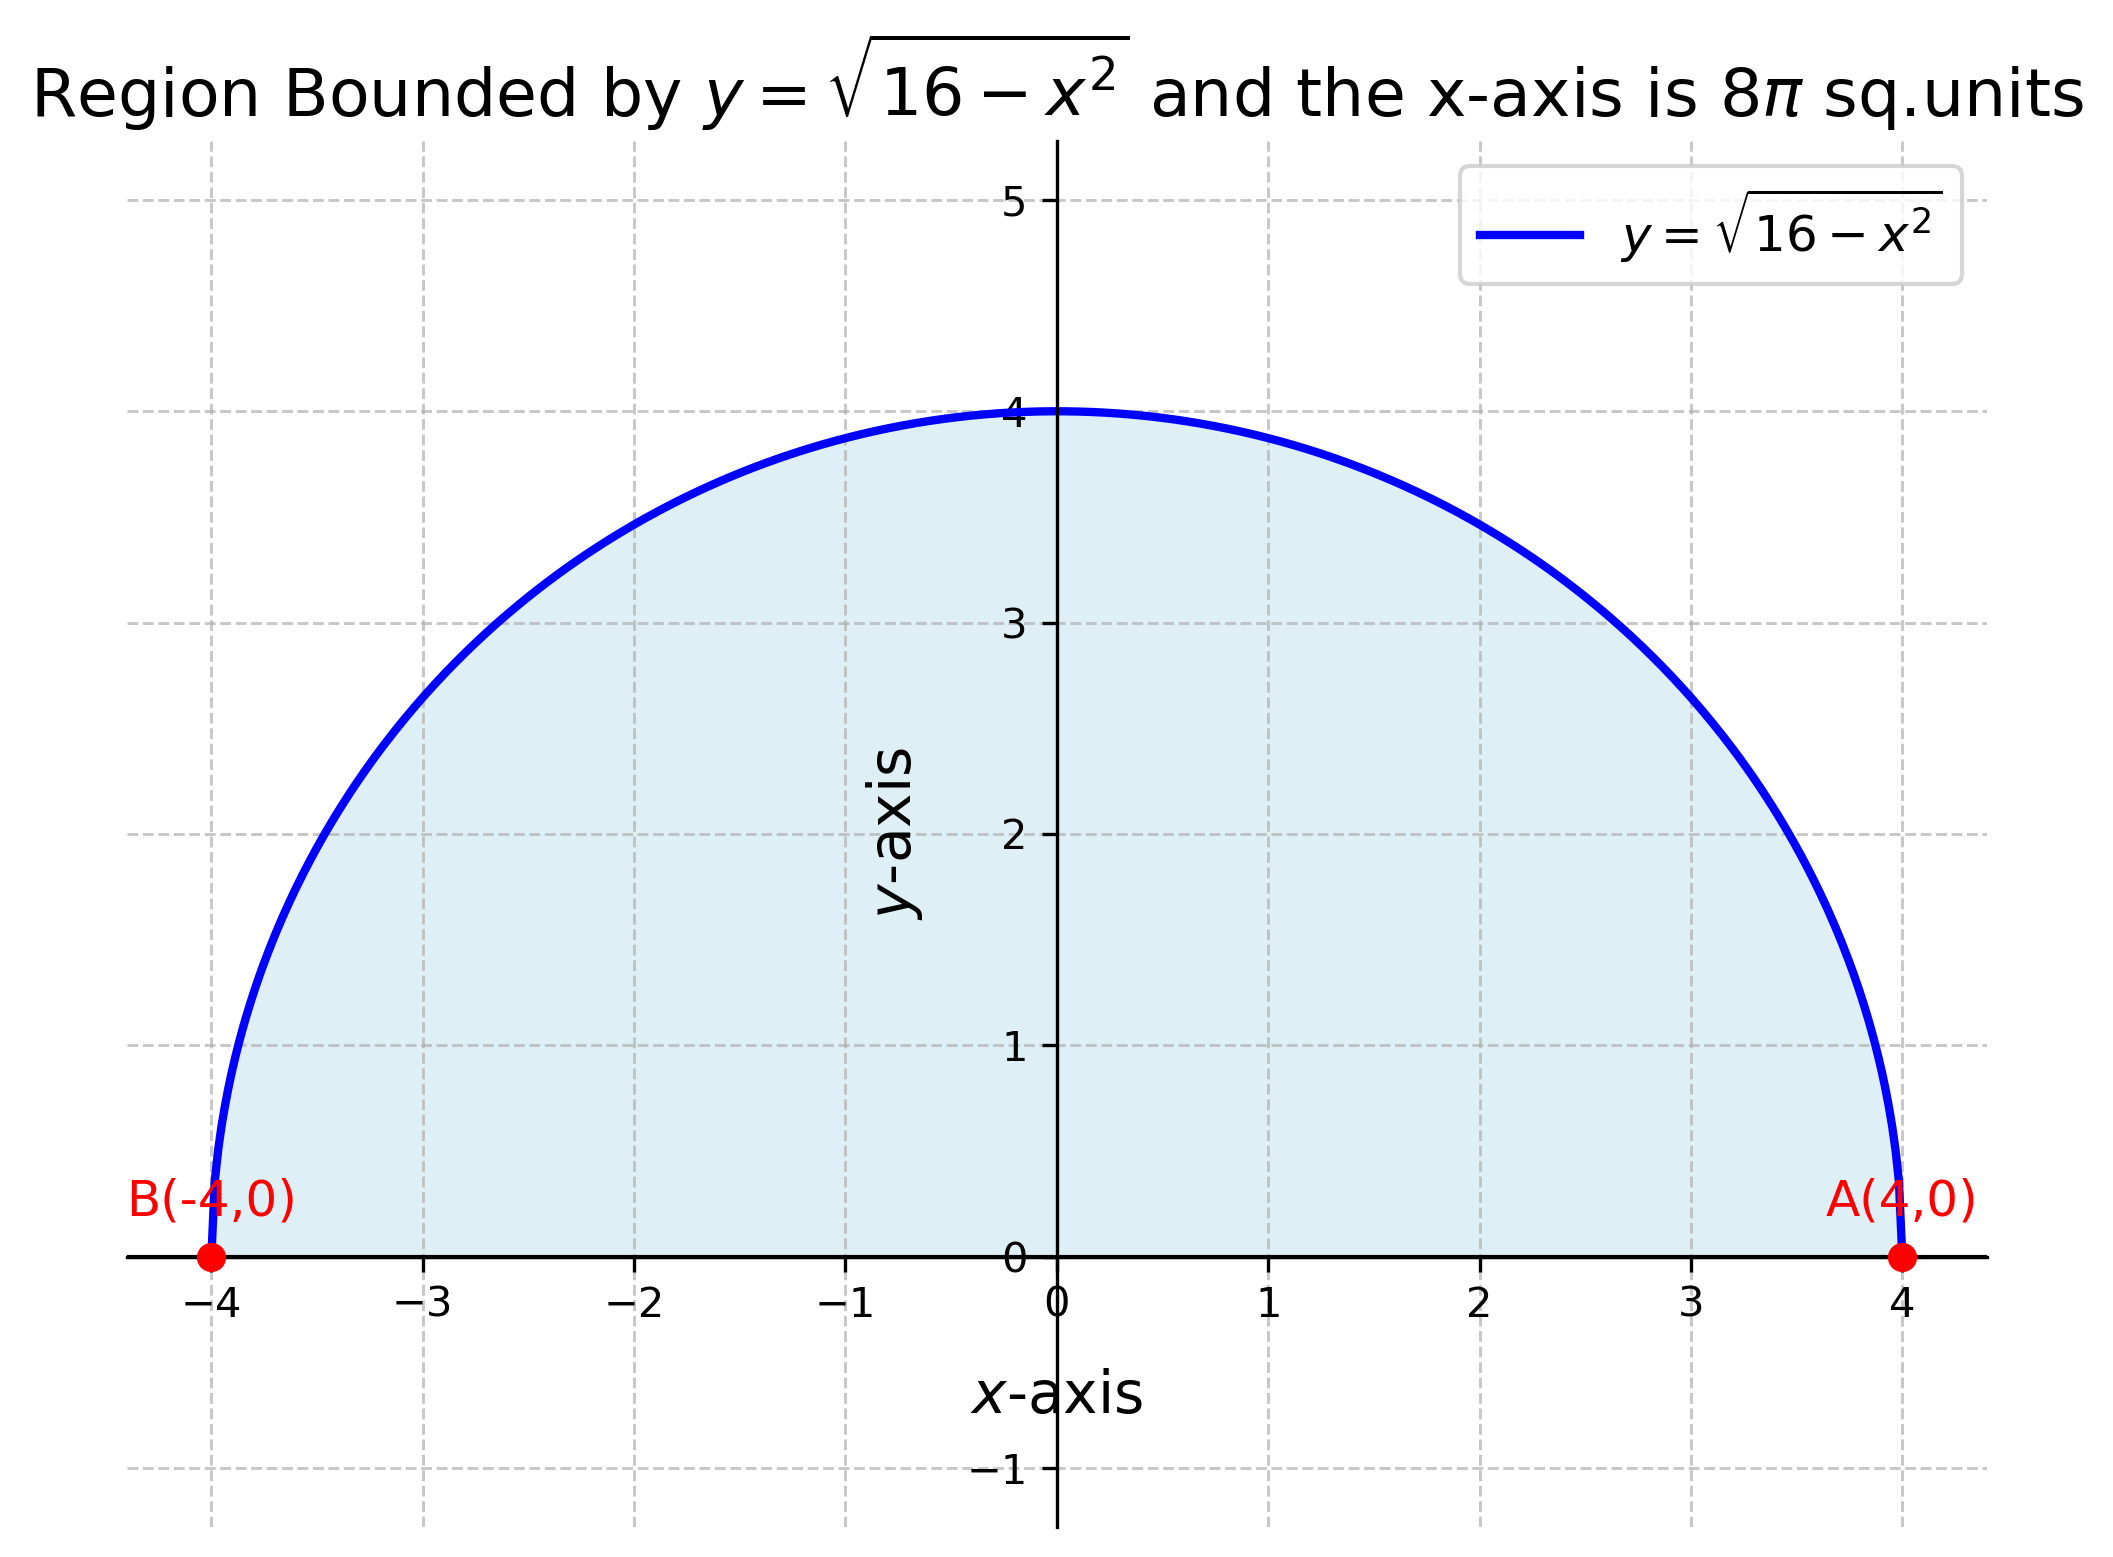
\includegraphics[scale=0.7]{figs/plot.png}
	\label{Fig}
\end{figure}


\end{document}
